%        File: arfc-beamer.tex
%     Created: Sun May 5 10:00 PM 2013 C
%


%\documentclass[11pt,handout]{beamer}
\documentclass[9pt]{beamer}
\usetheme[white]{Illinois}
%\title[short title]{long title}
\title[OpenMC transport independent depletion]{Burning fuel for cheap!
Transport independent depletion in OpenMC}
%\subtitle[short subtitle]{long subtitle}
\author[Oleksandr Yardas]{Oleksandr Yardas\\Advanced Reactors and Fuel Cycles Group}
%\date[short date]{long date}
\date[07.09.2025]{July 9, 2025}
%\institution[short name]{long name}
\institute[UIUC]{University of Illinois at Urbana-Champaign}

%\usepackage{bbding}
\usepackage{amsfonts}
\usepackage{amsmath}
\usepackage{xspace}
\usepackage{graphicx}
\usepackage{subfig}
\usepackage{booktabs} % nice rules for tables
\usepackage{microtype} % if using PDF
\usepackage{bigints}
\usepackage{minted}
\usepackage[version=4]{mhchem} % nuclide symbols

\newcommand{\units}[1] {\:\text{#1}}%
\newcommand{\SN}{S$_N$}%{S$_\text{N}$}%{$S_N$}%
\DeclareMathOperator{\erf}{erf}
%I need some complimentary error functions...
\DeclareMathOperator{\erfc}{erfc}
%Those icons in the references are terrible looking
\setbeamertemplate{bibliography item}[text]

%%%% Acronym support

\usepackage[acronym,toc]{glossaries}
\include{acros}

\makeglossaries

%try to get rid of header on title page\dots
\makeatletter
    \newenvironment{withoutheadline}{
        \setbeamertemplate{headline}[default]
        \def\beamer@entrycode{\vspace*{-\headheight}}
    }{}
\makeatother

\makeatother
\setbeamertemplate{footline}
{
  \leavevmode%
  \hbox{%
    \rightline{\insertframenumber{} / \inserttotalframenumber\hspace*{1ex}}
  }%
  \vskip0pt%
}
\makeatletter
% This will add figure numbers to captions.
\setbeamertemplate{caption}[numbered]

\begin{document}
%%%%%%%%%%%%%%%%%%%%%%%%%%%%%%%%%%%%%%%%%%%%%%%%%%%%%%%%%%%%%
%% From uw-beamer Here's a handy bit of code to place at
%% the beginning of your presentation (after \begin{document}):
\newcommand*{\alphabet}{ABCDEFGHIJKLMNOPQRSTUVWXYZabcdefghijklmnopqrstuvwxyz}
\newlength{\highlightheight}
\newlength{\highlightdepth}
\newlength{\highlightmargin}
\setlength{\highlightmargin}{2pt}
\settoheight{\highlightheight}{\alphabet}
\settodepth{\highlightdepth}{\alphabet}
\addtolength{\highlightheight}{\highlightmargin}
\addtolength{\highlightdepth}{\highlightmargin}
\addtolength{\highlightheight}{\highlightdepth}
\newcommand*{\Highlight}{\rlap{\textcolor{HighlightBackground}{\rule[-\highlightdepth]{\linewidth}{\highlightheight}}}}
%%%%%%%%%%%%%%%%%%%%%%%%%%%%%%%%%%%%%%%%%%%%%%%%%%%%%%%%%%%%%
%%--------------------------------%%
\begin{withoutheadline}
\frame{
  \titlepage
}
\end{withoutheadline}

%%--------------------------------%%
\AtBeginSection[]{
\begin{frame}
  \frametitle{Outline}
  \tableofcontents[currentsection]
\end{frame}
}

\section{Motivation}
\subsection{The Computer Problem}
\begin{frame}
  \frametitle{Simulating a nuclear reactor is expensive!}
  \begin{itemize}
      \item Seven dimensions: space (3), energy (1) angle (2), time (1)
      \item Low-error $\rightarrow$ computationally-intensive methods
  \end{itemize}

  \begin{figure}[htpb]
           \centering
           
\includegraphics[width=5cm]{./images/atr.png} 
           \caption{OpenMC model of the ATR Reactor, from \cite{openmc_atr_slice}}
           \label{fig:atr}
  \end{figure}
\end{frame}

\subsection{Nuclear Basics}
\begin{frame}
  \frametitle{Fission Chain Reaction}
  % a comment
  \begin{figure}[htbp!]
    \begin{center}
      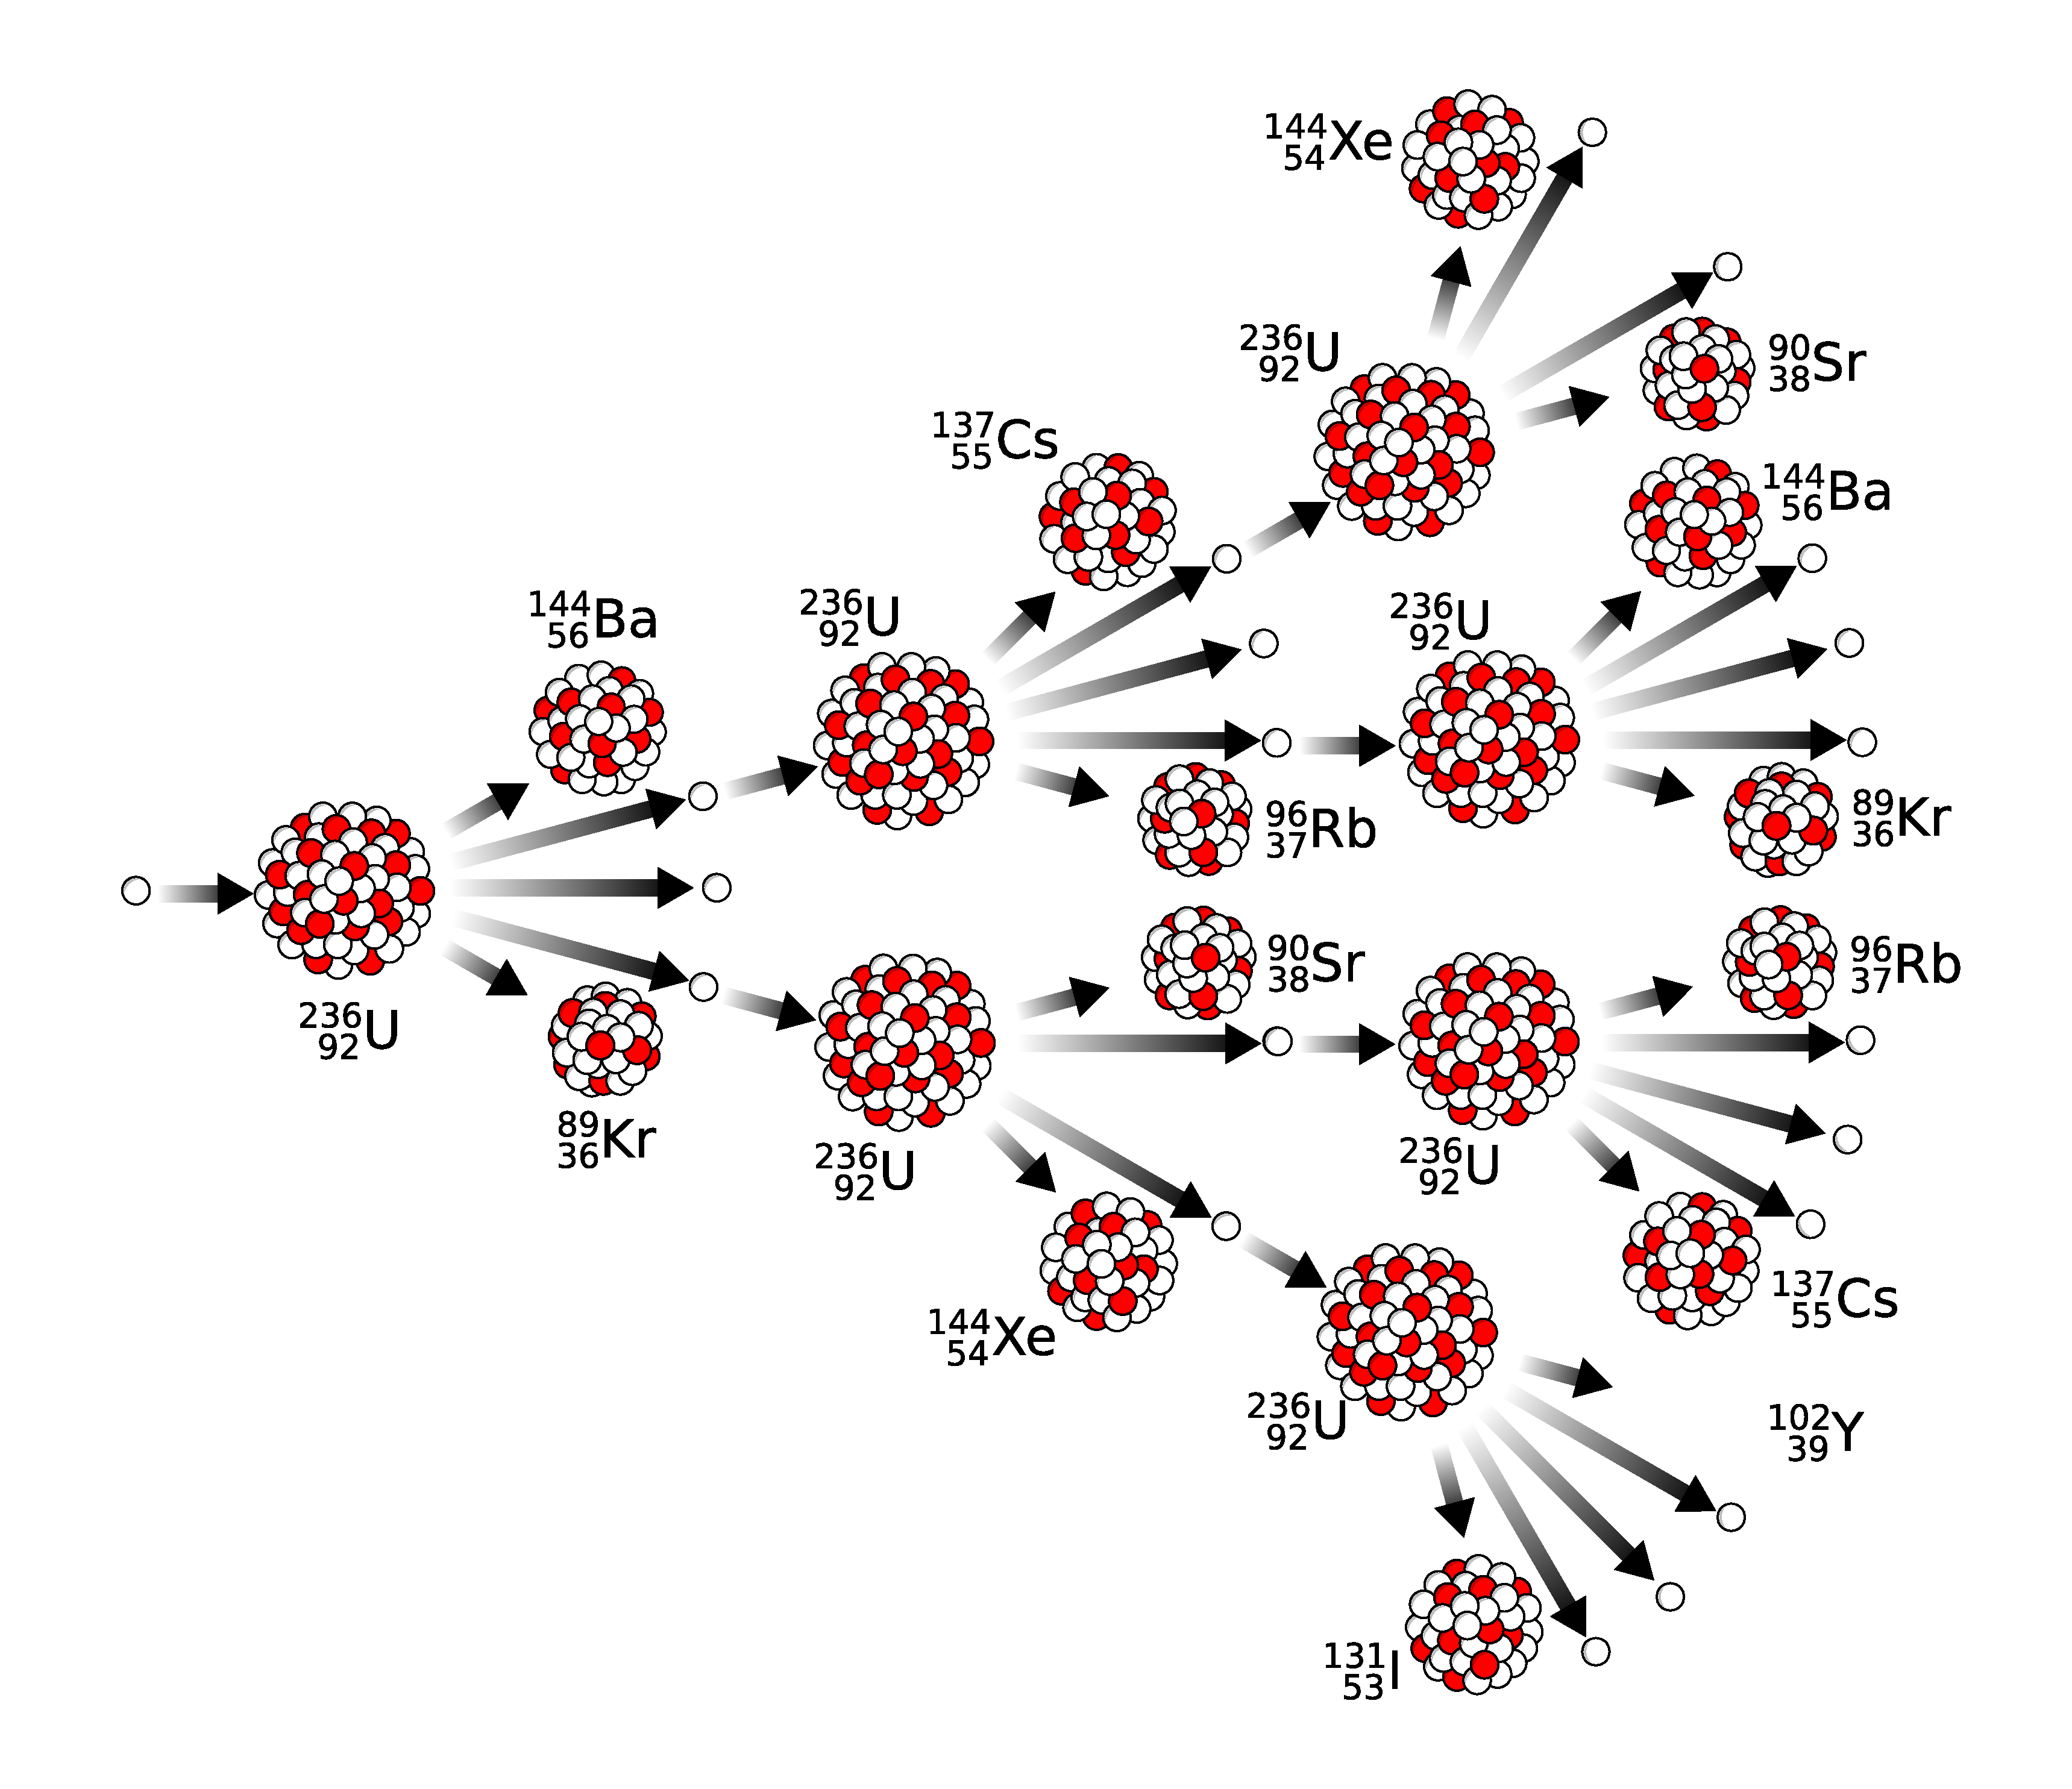
\includegraphics[height=6cm]{./images/Nuclear_fission_chain_reaction.pdf}
    \end{center}
          \caption{Diagram of a fission chain reaction, from
          \cite{nuclear_wikipedia_2017}.}
    \label{fig:fisson-reaction}
  \end{figure}
\end{frame}

\begin{frame}
    \frametitle{Depletion}
        \begin{columns}
            \column[t]{5cm}
                From Duderstadt \& Hamilton, Nuclear Reactor Analysis:
                \begin{quote}
                        The atomic densities of various isotopes in a reactor
                        core are continually changing due to niclear processes
                        such as fission, neutron capture, and radioactive decay
                \end{quote}
                

                Why do we care?
            \column[t]{5cm}
                \begin{figure}[htbp!]
                    \begin{center}
                        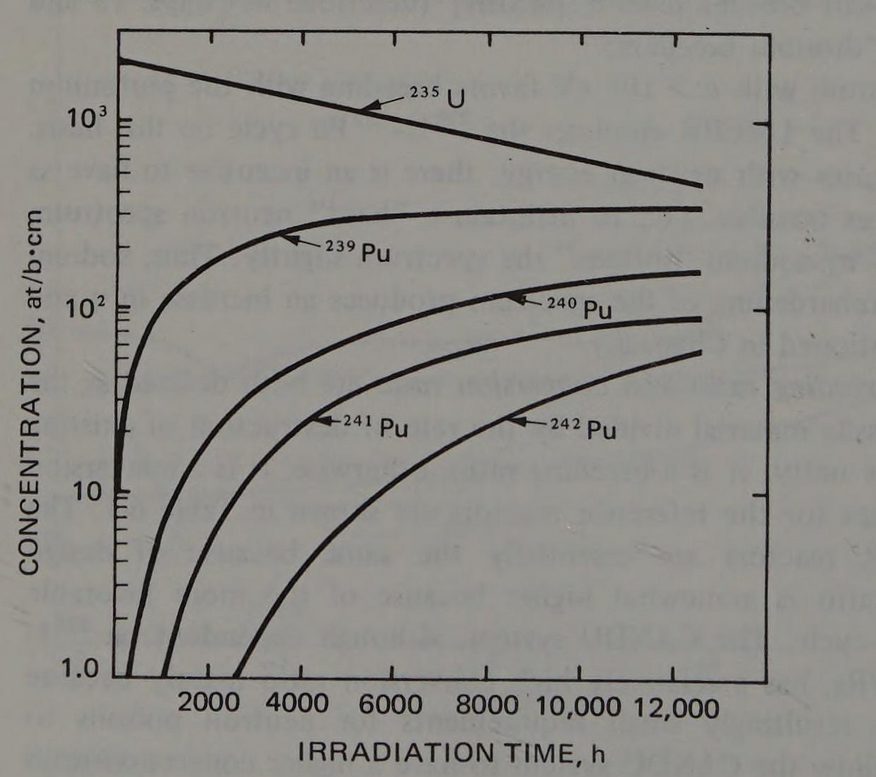
\includegraphics[height=5cm]{./images/isotopes_over_time.png}
                    \end{center}
                    \caption{Buildup of plutionium isotopes with a burnup for a
                    typical LWR fuel composition. Reproduced from Figure 6-2 in
                    \cite{knief_nuclear_1981}.}
                    \label{fig:isotopes-over-time}
                \end{figure}
        \end{columns}
\end{frame}

\begin{frame}
    \frametitle{Depletion makes everything {\it more} expensive}     
        \begin{columns}
            \column[t]{5cm}
               \begin{itemize}
                    \item Thousands of nuclides
                    \item Rections must be stored
                    \item Compositions must be stored
                \end{itemize}

                \begin{figure}[htbp]
                    \begin{center}
                        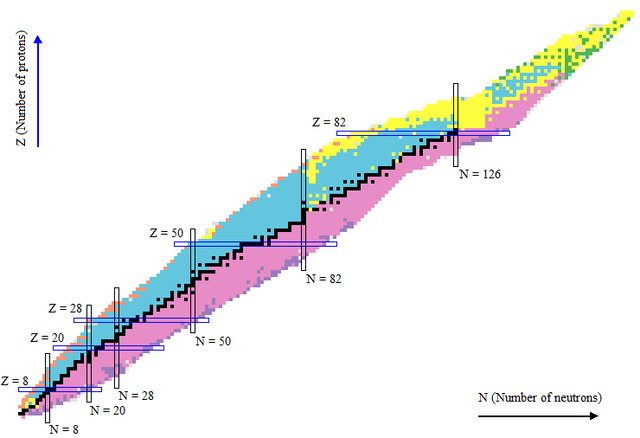
\includegraphics[height=3cm]{./images/nuclide_table.jpg}
                    \end{center}
                    \caption{Table of Nuclides. Z on y-axis, N on x-axis. From
                    \cite{tracy_jr_binding_2017}}
                    \label{fig:nuclide-table}
                \end{figure}
            \column[t]{5cm}
                \begin{figure}[htbp]
                    \begin{center}
                        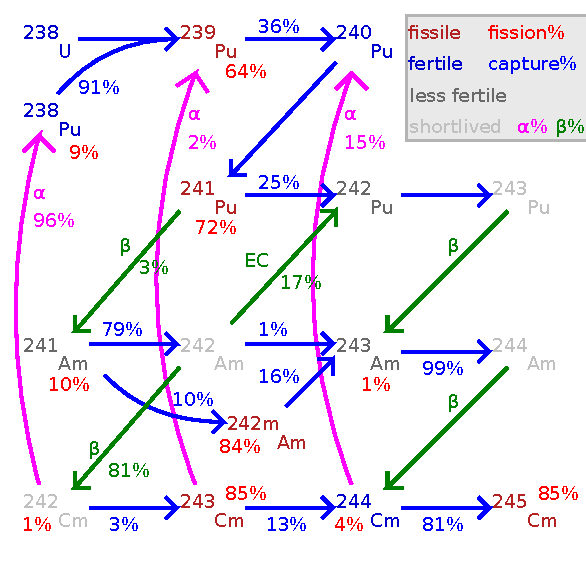
\includegraphics[height=5cm]{./images/pu-chain.pdf}
                    \end{center}
                    \caption{Example of the complicated web of production and
                    transmutation reactions. From \cite{wikipedia_magyar_2007}}
                    \label{fig:pu-chain}
                \end{figure}
        \end{columns}
\end{frame}



\section{Methods}
\subsection{Modeling Depletion}
\begin{frame}
  \frametitle{Modeling Depletion}
  Governing Equation:
    \begin{equation}
      \label{eq:depletion}
      \begin{split}
          \frac{dN_i}{dt} = & \sum\limits_{j=1}^n \overbrace{N_j(t)\int_0^\infty
            f_{j \rightarrow i}(E) \sigma_j (E) \phi(E,t) dE}^\text{Production
            of $i$ from $j$} \;+
          \sum\limits_{j=1}^n \overbrace{N_j(t) \lambda_{j\rightarrow
            i}}^\text{Decay of $j$ into $i$}
          \\ & - N_i(t)\underbrace{\int_0^\infty \sigma_i (E) \phi(E,t)
            dE}_\text{Consumption of $i$} \; -
          \underbrace{N_i(t)\sum\limits_{j=1}^n \lambda_{i\rightarrow
            j}}_\text{Decay of $i$} ,
      \end{split}
    \end{equation}
    where
    \begin{equation*}
      \begin{split}
          N_i(t) &\equiv \text{density of nuclide $i$ at time $t$ [cm$^{-3}$]}\\
        \sigma_i(E,t) &\equiv \text{transmutation cross section for nuclide $i$ at energy $E$ and time $t$ [cm$^{2}$]}\\
            \phi(E,t) &\equiv \text{neutron flux at energy $E$ and time $t$ [n
            cm$^{-2}$ s$^{-1}$]} \\
        f_{j \rightarrow i}(E) &\equiv \text{fraction of transmutation reactions in nuclide $j$ that produce nuclide $i$} \\
        \lambda_{j \rightarrow i} &\equiv \text{decay constant for decay modes
        in nuclide $j$ that produce nuclide $i$ [s$^{-1}$]}\\
        n &\equiv \text{total number of nuclides.}
      \end{split}
    \end{equation*}
\end{frame}

\begin{frame}
    \frametitle{Modeling Depletion (continued)}
    \begin{block}{What do we need to solve Equation \ref{eq:depletion}?}
      \begin{itemize}
          \item $N_{i}(t),\; n\; \rightarrow$ Given by the problem (e.g.
              Westinghouse PWR using 5\% enriched fuel at BOL)
          \item $\sigma_{i}(E,t),\;f_{j\rightarrow i},\; \lambda_{j \rightarrow
              i}\; \rightarrow$ Material properties (data stored in memory
              for speed)
          \item $\phi(E,t)\; \rightarrow$ Concentration of neutrons in the
              reactior; requires a neutron transport simulation
      \end{itemize}  
    \end{block}
    
    \begin{block}{Can we make this cheaper?}
        \pause
        Assume {\it static} fluxes $\rightarrow$ decouple transport from
        depletion.
    \end{block}
\end{frame}

\subsection{Code Additions}
\begin{frame}
  \frametitle{Neutron transport software of choice: OpenMC}
  \begin{figure}[htpb]
      \centering
      
\includegraphics[width=0.8\textwidth]{./images/openmc_logo.png}
  \end{figure}
  \begin{itemize}
      \item Monte carlo code
      \item Open source, community developed!!
      \item NumPy, H5Py, Pandas, Matplotlib, SciPy(!!), uncertainties
  \end{itemize}
\end{frame}

\begin{frame}
  \frametitle{OpenMC's depletion module}
  \begin{enumerate}
      \item Run an OpenMC simulation and get reaction rates for all nuclides
          with available data (C++)
      \item Process reactions information to solve Equation
          \ref{eq:depletion} (numpy for vectors and dense arrays, scipy for
          sparse arrays)
      \item Update material compositions and rerun
      \item Repeat for all time steps
  \end{enumerate}
\end{frame}

\begin{frame}
  \frametitle{Machinery to support static cross sections and fluxes}
    \begin{columns}
            \column[t]{5cm}
                \begin{block}{MicroXS}
                    \begin{itemize}
                        \item Stores $\sigma_{i,g} \rightarrow$ discretized on an energy grid
                        \item Indexed by nuclide, reaction name, energy group
                    \end{itemize}
                \end{block}

                \begin{block}{get\_microxs\_and\_flux()}
                    \begin{itemize}
                        \item Run an OpenMC simulation to obtain $\sigma_{i,g}$
                            and $\phi_{g}$ for all nuclides i (one material)
                        \item Can get $\sigma_{i,g},; \phi_{g}$ for as many
                            materials/domains as desired
                        \item $\phi_{g} \rightarrow$ Static fluxes discretized on an
                            energy grid
                    \end{itemize}
                \end{block}
            \column[t]{5cm}
                \begin{block}{IndependentOperator}
                    \begin{itemize} 
                        \item Drop in replacement for Operator class
                        \item Multiply $\phi_{g}$ and $N_{i}(t) \sigma_{i,g}$ to
                            to get reaction rate for nuclide $i$
                    \end{itemize}
                \end{block}
    \end{columns}
    \begin{center}
    \end{center}
\end{frame}

\subsection{Model Problem}
\begin{frame}
    \frametitle{Model Problem}
    \begin{columns}
            \column[t]{5cm}
            \begin{itemize}
                \item Single \Gls{PWR} pincell
                \item 4.25\% enriched fuel
                \item Reflective boundary conditions
            \end{itemize}
            Three cases:
            \begin{enumerate}
                \item Transport-coupled depletion (base truth)
                \item Transport-independent depletion
                \item Transport-independent depletion w/ recalculated cross sections
                    (sanity check)
            \end{enumerate}
            Ten time steps, two different $\Delta$t:
            \begin{enumerate}
                \item 3-day (Xe 135 poisioning limit)
                \item 30-day (long timestep approximation)
            \end{enumerate}
            \column[t]{5cm}
                \begin{figure}[htpb]
                    \centering
                    
\includegraphics[width=0.8\textwidth]{./images/pincell.png}
                    \caption{Slice plot of the pincell model in the
                    $xy$-plane. Blue = water, black = cladding, pink = fuel}
                    \label{fig:pincell}
                \end{figure}
            Three energy group structures:
                One group (single energy),
                8 group,
                40 group

    \end{columns}
\end{frame}

\section{Results}
\begin{frame}
    \frametitle{Run time}
    Explicit run time data was not collected, but based on the file timestamps,
    we can estimate how long each case took to complete on a cluster
    \begin{table}[htpb]
        \centering
        \caption{Comparison of average total runtimes}
        \label{tab:label}
        \begin{tabular}{|c|c|p{0.5\linewidth}|}
         Case & Runtime scale & Notes\\
         1 & hours &  \\
         2 & minutes & Does not include the initial simulation to obatin $\phi_{g}$
         and $\sigma_{i,g}$ \\
         3 & hours & Cross section data had to be loaded in at each timestep, s
         this case took the longest amount of time
        \end{tabular}
    \end{table}
    Case 2 is {\it very} fast!
\end{frame}

\begin{frame}
    \frametitle{One-group actinides (3-day time steps)}
    \begin{figure}[htpb]
        \centering
        \subfloat[] {
            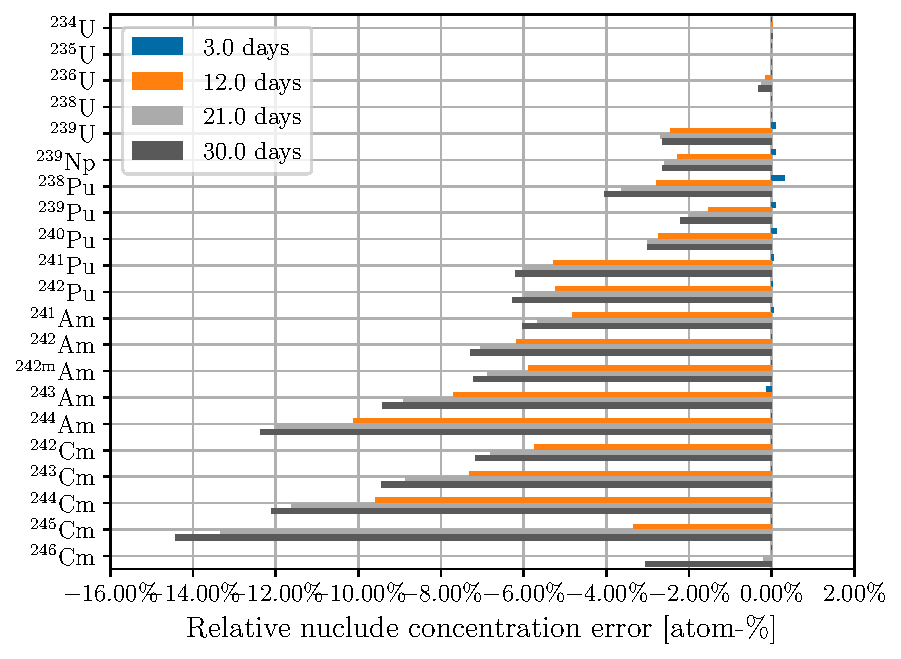
\includegraphics[width=0.5\linewidth]{./../paper/figs/actinides_constant_xs_predictor_fission_q_days.pdf}
            \label{fig:actinides-error-constant-xs-days}
        }
        \subfloat[] {
            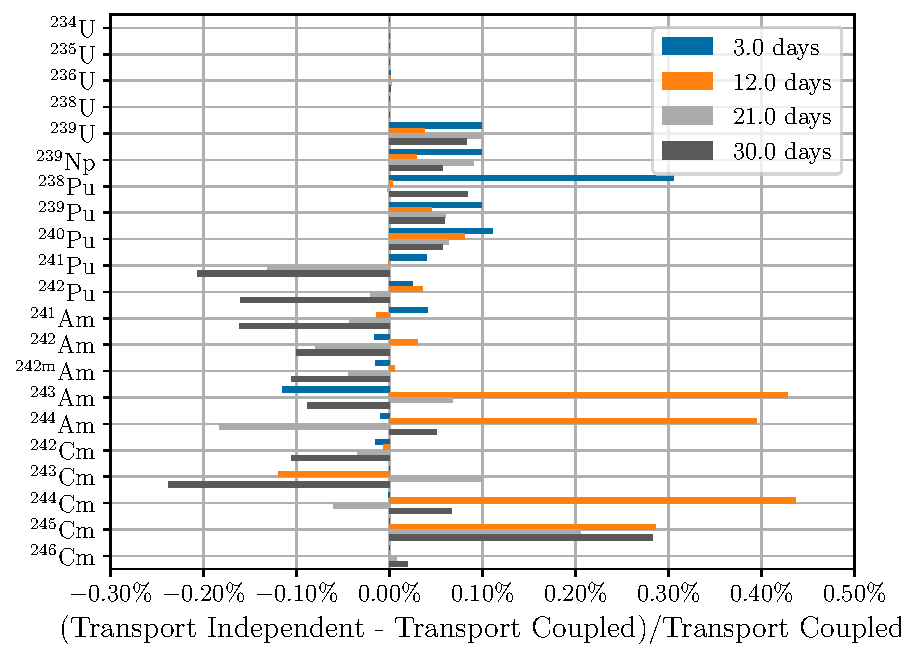
\includegraphics[width=0.5\linewidth]{./../paper/figs/actinides_updating_xs_predictor_fission_q_days.pdf}
            \label{fig:actinides-error-updating-xs-days}
        }
        \caption[]{Actinide concentration error relative to Case 1 using 3-day time steps at 3,
                12, 21, and 30 days of depletion for
            \subref{fig:actinides-error-constant-xs-days} constant cross
            sections (Case 2);
            \subref{fig:actinides-error-updating-xs-days} updating cross
            sections (Case 3).}
    \end{figure}
\end{frame}

\begin{frame}
    \frametitle{One-group actinides (30-day time steps)}
    \begin{figure}[h!tpb]
        \centering
        \subfloat[] {
            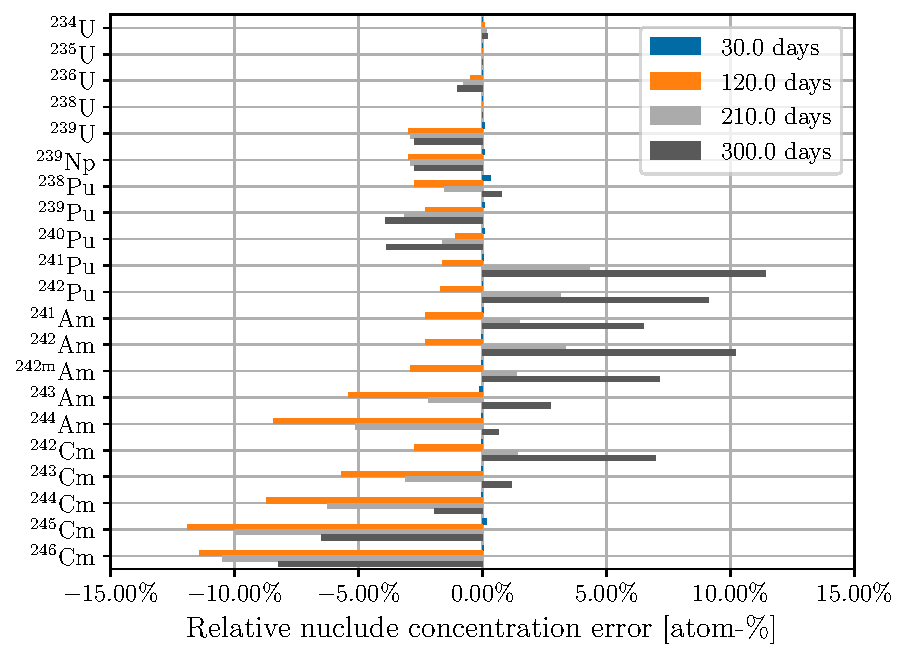
\includegraphics[width=0.5\linewidth]{./../paper/figs/actinides_constant_xs_predictor_fission_q_months.pdf}
            \label{fig:actinides-error-constant-xs-months}
        }
        \subfloat[] {
            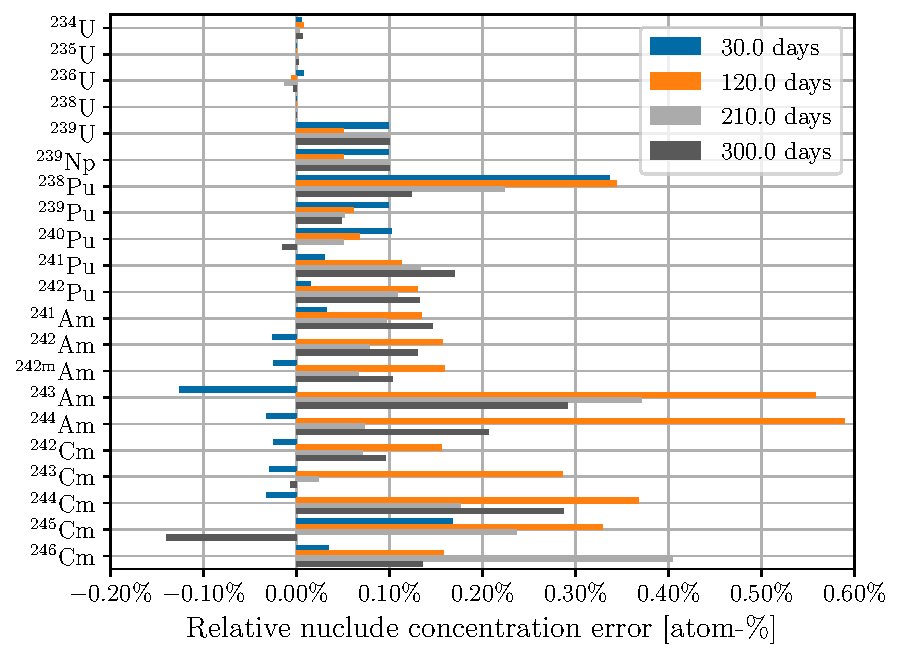
\includegraphics[width=0.5\linewidth]{./../paper/figs/actinides_updating_xs_predictor_fission_q_months.pdf}
            \label{fig:actinides-error-updating-xs-months}
        }
        \caption[]{Actinide concentration error relative to Case 1 using 30-day time steps
            at 30,
                120, 210, and 300 months of depletion for
            \subref{fig:actinides-error-constant-xs-months} constant cross
            sections (Case 2);
            \subref{fig:actinides-error-updating-xs-months} updating cross
            sections (Case 3).}
    \end{figure}
\end{frame}

\begin{frame}
    \frametitle{Overprediction of $(n,\gamma)$ reaction rates on \ce{^{240}Pu}}
    \begin{figure}[htpb]
        \centering
        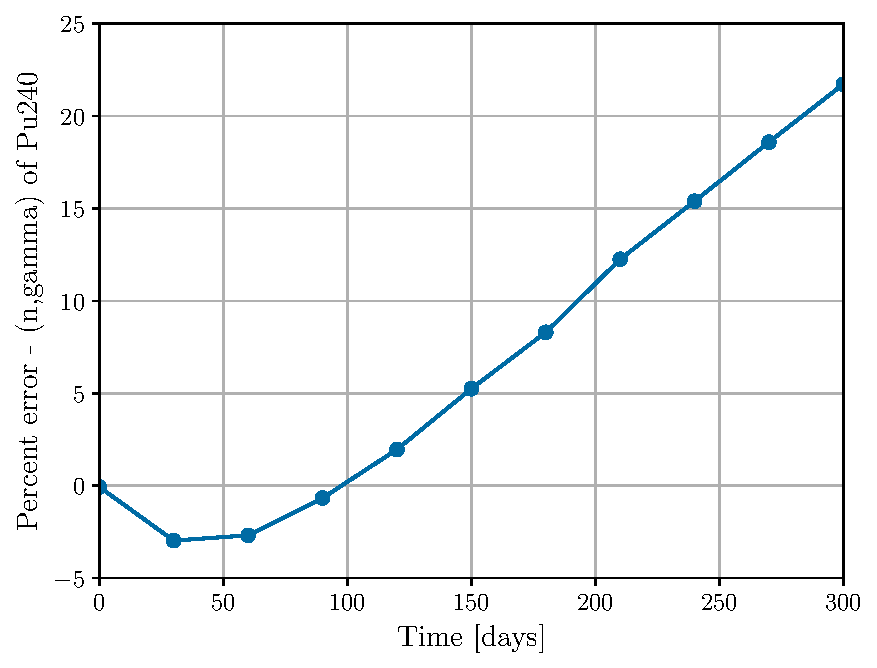
\includegraphics[width=0.5\linewidth]{./../paper/figs/pu240-n-gamma-months.pdf}
        \caption{Relative \ce{^{240}Pu} ($n,\gamma$) reaction rate error using
        constant cross sections and 30-day time steps.}
        \label{fig:pu240-n-gamma-months}
    \end{figure}
\end{frame}



\begin{frame}
    \frametitle{Fission products (3-day time steps)}
    \begin{figure}[h!tpb]
        \centering
        \subfloat[] {
            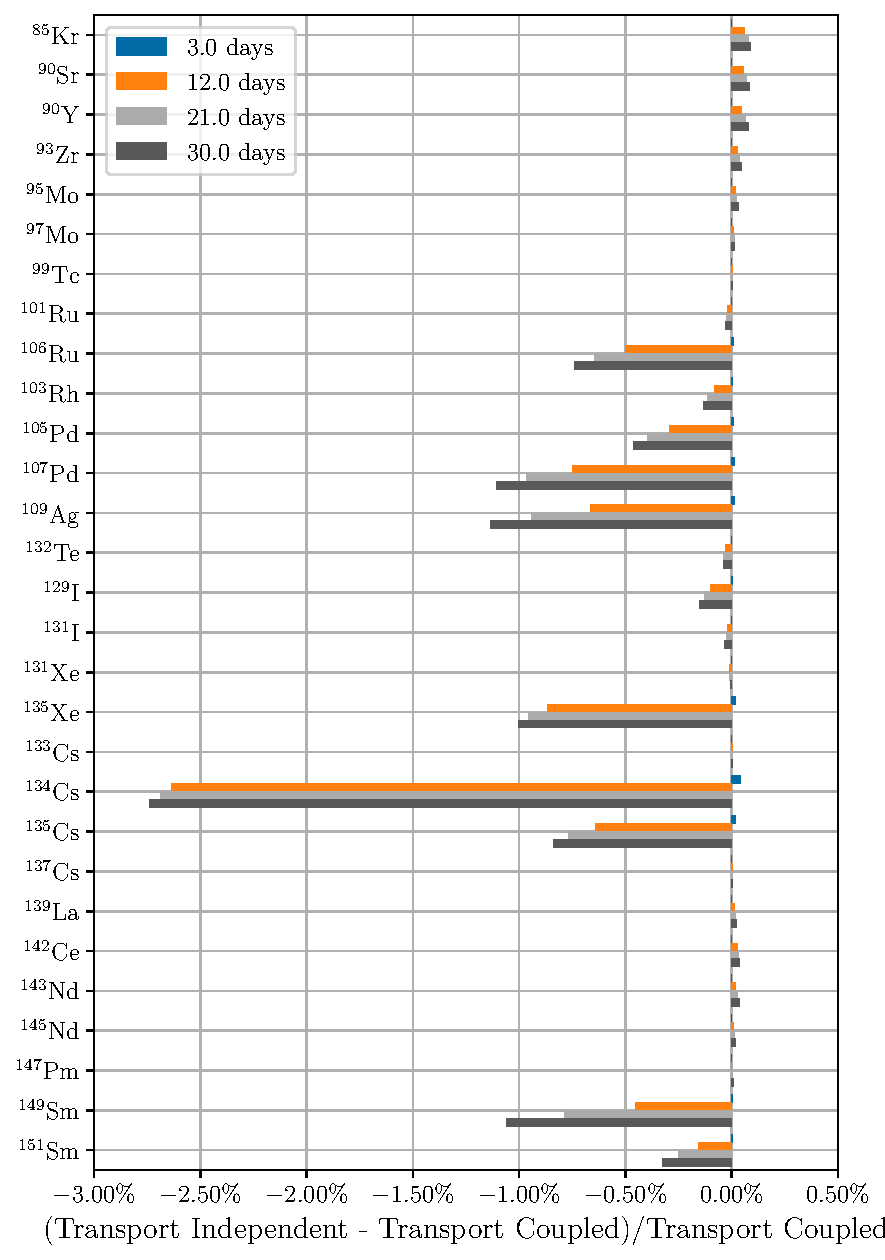
\includegraphics[width=0.4\linewidth]{./../paper/figs/fission_products_constant_xs_predictor_fission_q_days.pdf}
            \label{fig:fp-error-constant-xs-days}
        }
        \subfloat[] {
            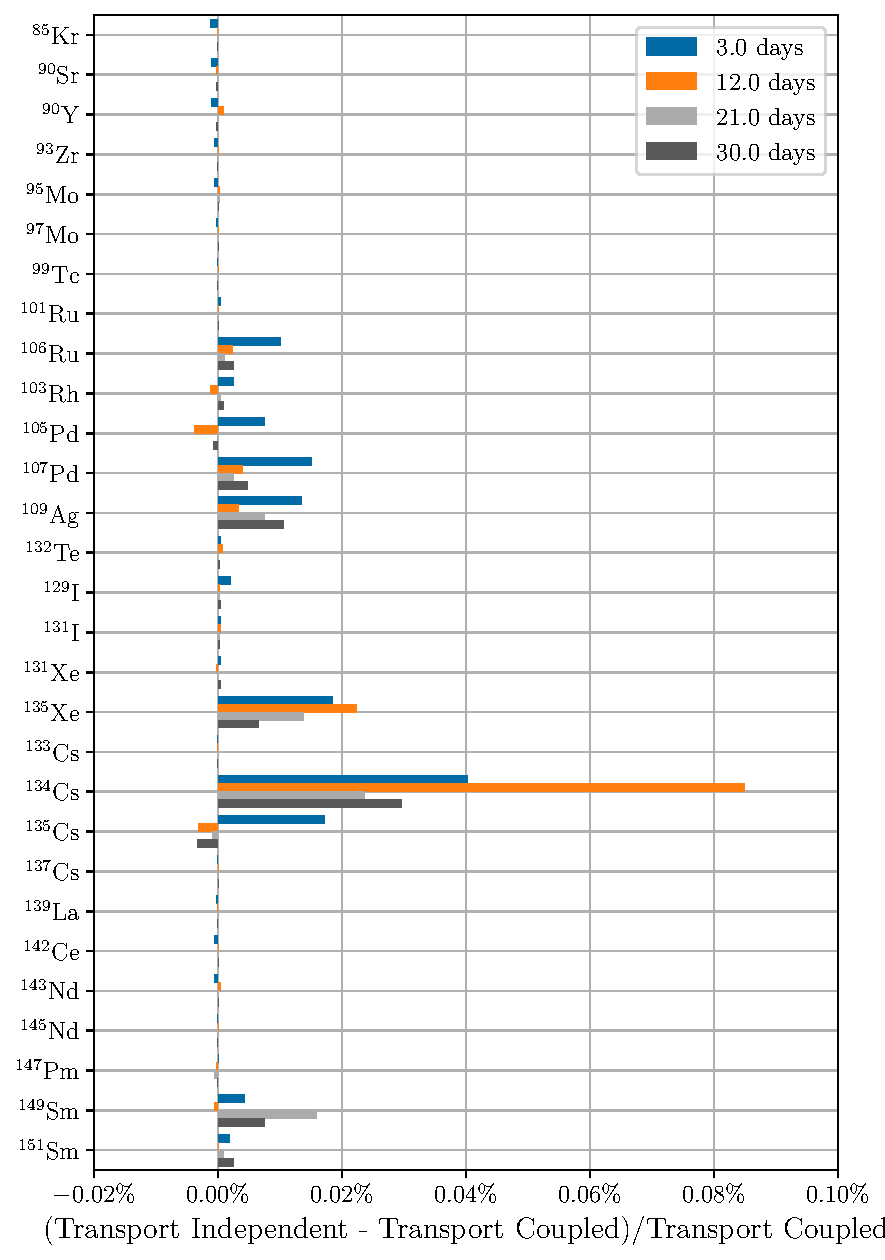
\includegraphics[width=0.4\linewidth]{./../paper/figs/fission_products_updating_xs_predictor_fission_q_days.pdf}
            \label{fig:fp-error-updating-xs-days}
        }
        \caption[]{\subref{fig:fp-error-constant-xs-days} constant cross
            sections (Case 2);
            \subref{fig:fp-error-updating-xs-days} updating cross sections (Case
        3).}
    \end{figure}
\end{frame}

\begin{frame}
    \frametitle{Fission products (30-day time steps)}
    \begin{figure}[h!tpb]
        \centering
        \subfloat[] {
            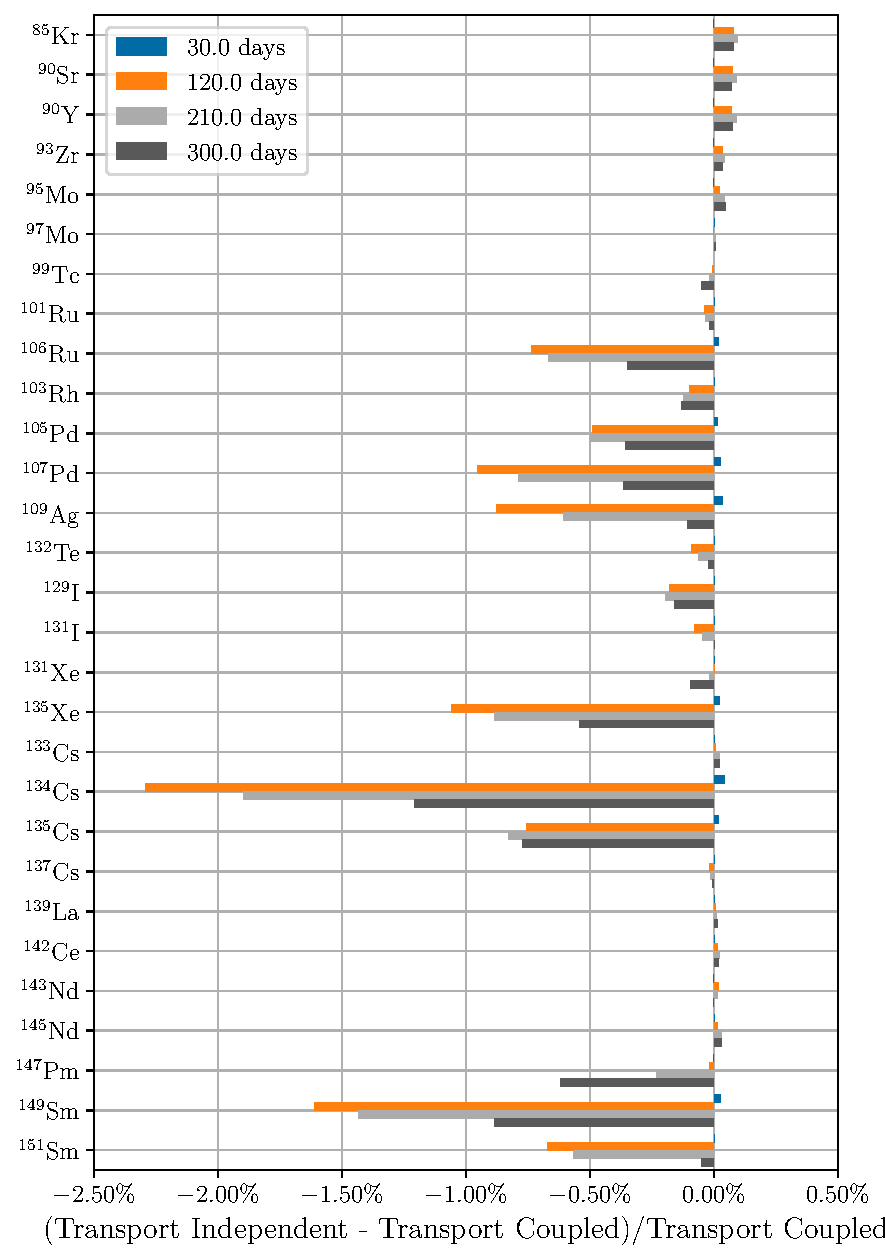
\includegraphics[width=0.4\linewidth]{./../paper/figs/fission_products_constant_xs_predictor_fission_q_months.pdf}
            \label{fig:fp-error-constant-xs-months}
        }
        \subfloat[] {
            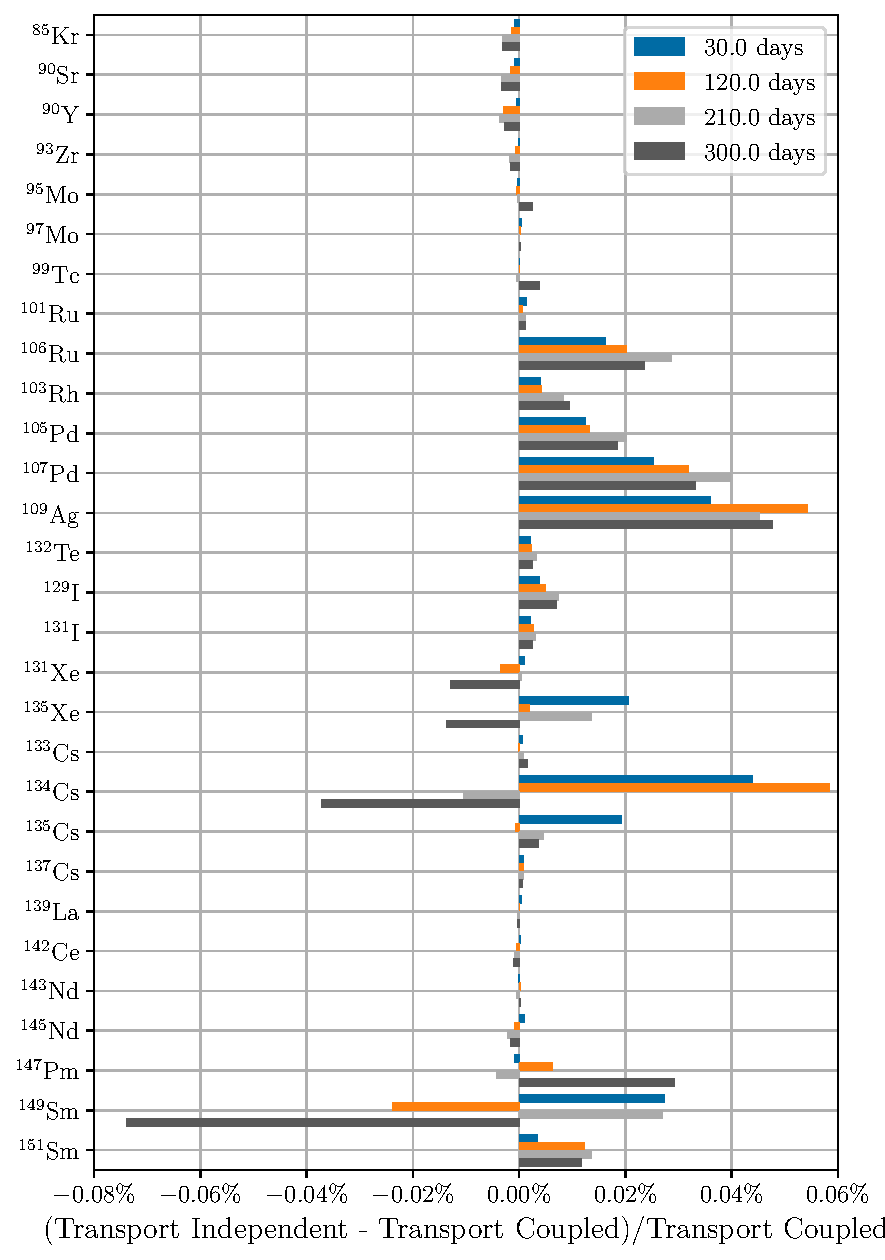
\includegraphics[width=0.4\linewidth]{./../paper/figs/fission_products_updating_xs_predictor_fission_q_months.pdf}
            \label{fig:fp-error-updating-xs-months}
        }
        \caption[]{\subref{fig:fp-error-constant-xs-months} constant cross
            sections (Case 2);
            \subref{fig:fp-error-updating-xs-months} updating cross sections
        (Case 3).}
    \end{figure}
\end{frame}

\begin{frame}
    \frametitle{8-group actinides}
    \begin{figure}[htpb]
        \centering
        \subfloat[] {
            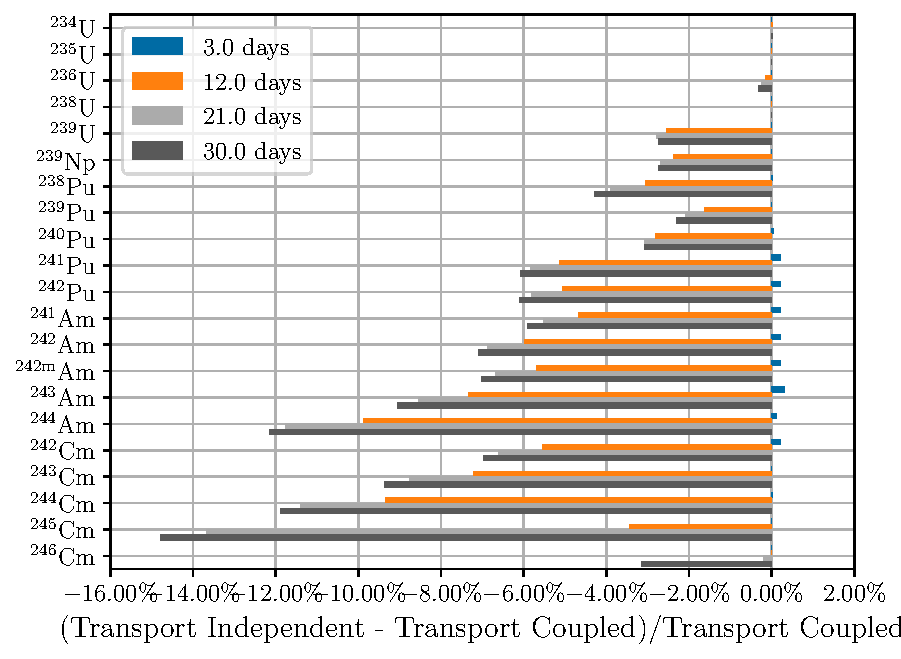
\includegraphics[width=0.5\linewidth]{./../paper/figs/actinides_casmo8_constant_xs_predictor_fission_q_days.pdf}
            \label{fig:actinides-error-casmo8-xs-days}
        }
        \subfloat[] {
            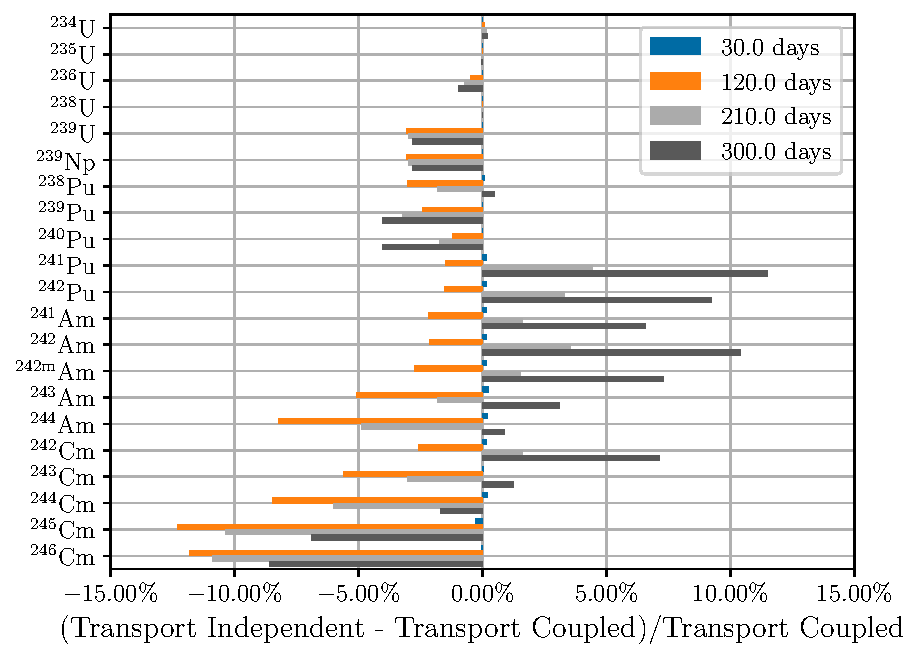
\includegraphics[width=0.5\linewidth]{./../paper/figs/actinides_casmo8_constant_xs_predictor_fission_q_months.pdf}
            \label{fig:actinides-error-casmo8-xs-months}
        }
        \caption[]{
            \subref{fig:actinides-error-casmo8-xs-days} 3-day time steps;
            \subref{fig:actinides-error-casmo8-xs-months} 30-day time steps}
    \end{figure}
\end{frame}

\begin{frame}
    \frametitle{40-group actinides}
    \begin{figure}[htpb]
        \centering
        \subfloat[] {
            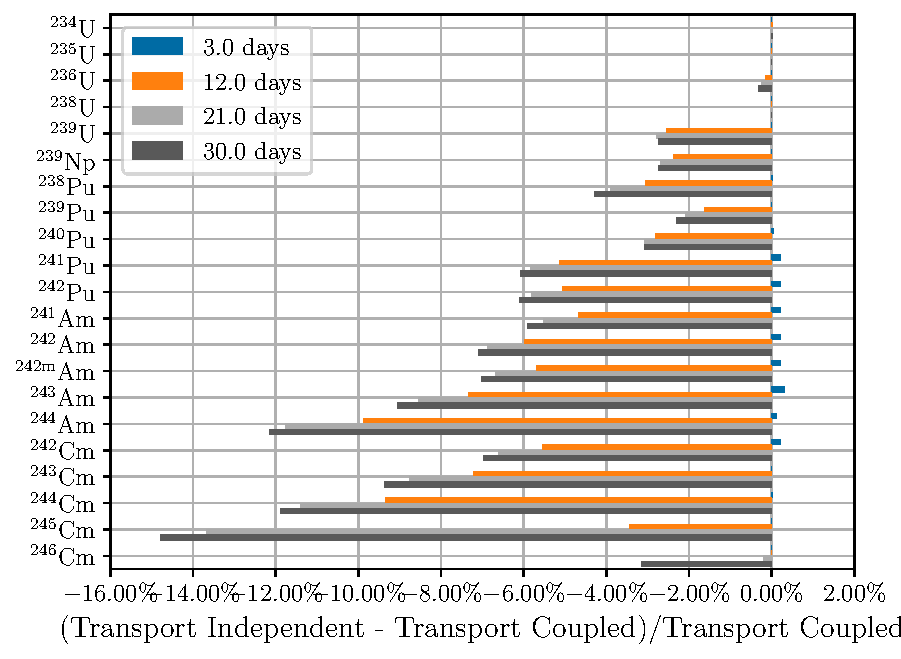
\includegraphics[width=0.5\linewidth]{./../paper/figs/actinides_casmo40_constant_xs_predictor_fission_q_days.pdf}
            \label{fig:actinides-error-casmo40-xs-days}
        }
        \subfloat[] {
            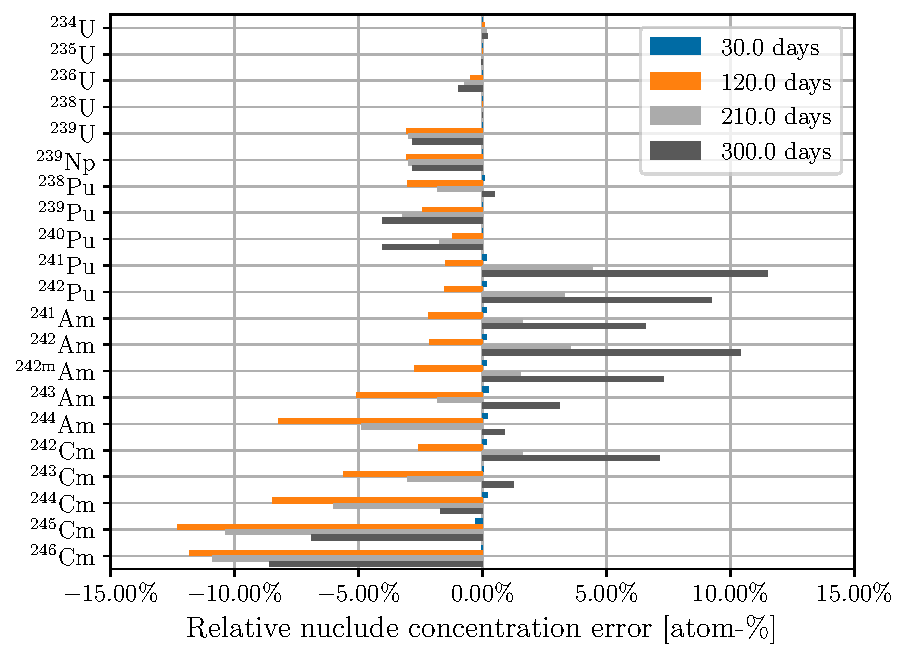
\includegraphics[width=0.5\linewidth]{./../paper/figs/actinides_casmo40_constant_xs_predictor_fission_q_months.pdf}
            \label{fig:actinides-error-casmo40-xs-months}
        }
        \caption[]{
            \subref{fig:actinides-error-casmo40-xs-days} 3-day time steps;
            \subref{fig:actinides-error-casmo40-xs-months} 30-day time steps}
    \end{figure}
\end{frame}

\section{Conclusion}
\begin{frame}
  \frametitle{Conclusion}
        \begin{itemize}
                \item Depletion calculations are expensive!                
                \pause
                \item Static, energy-discretized fluxes and cross sections yield
                    low errors for abundant nuclides, moderate errors for trace
                    nuclides
                \pause
                \item Transport-independent depletion provide orders of
                    magnitude of speedup for low errors for low to moderate
                    errors in nuclide concenrataion.
                \pause
                \item Energy group strucutre does not matter for simple models
        \end{itemize}
\end{frame}

\begin{frame}
  \frametitle{Technical Gaps and future work}
        \begin{itemize}
                \item Full core model                
                \item Multiple materials/depletion zones
            \end{itemize}
\end{frame}

\begin{frame}
  \frametitle{Acknowledgement}
  People:
  \begin{itemize}
      \item Paul Romano - Conceptualization, Methodology, Software, Funding acquisition, Writing - review and editing
      \item Madicken Munk and Kathryn Huff - Funding acquisition, Writing - review and editing 
  \end{itemize}

  Funding streams:
  \begin{itemize}
      \item Exascale Computing Project (17-SC-20-SC) (initial implementation)
      \item NRC Integrated University Grant Program Fellowship.
      \item U.S. Department of Energy Office of Fusion Energy Sciences Award Number DE-SC0022033.
  \end{itemize}

  Computing resources:
  \begin{itemize}
      \item Bebop (Argonne National Laboratory)
      \item Sawtooh (Idaho National Lab, Office of Nuclear Energy of the U.S.
          Department of Energy and the Nuclear Science User Facilities Contract
          No. DE-AC07-05ID14517)
  \end{itemize}
\end{frame}

%%--------------------------------%%
%%--------------------------------%%
\begin{frame}[allowframebreaks]
  \frametitle{References}
  \bibliographystyle{plain}
  {\footnotesize \bibliography{bibliography.bib} }

\end{frame}

%%--------------------------------%%


\end{document}



